\documentclass{article}
\usepackage{geometry}
\usepackage{longtable}
\usepackage{array}
\usepackage{lipsum}
\usepackage{listings}
\usepackage{graphicx}
\usepackage[italian,english]{babel}

\lstset{
    extendedchars=true,
    literate={ì}{{\`i}}1 {è}{{\`e}}1 {à}{{\`a}}1 {ò}{{\`o}}1 {ù}{{\`u}}1
}

\geometry{a4paper, margin=1in}

\title{Progetto DataBase}
\author{Mutua Fadhla Mohamed | SM3201434}
\date{\today}

% Configure listings package
\lstset{
    basicstyle=\ttfamily\small, % Set font style and size
    breaklines=true,            % Enable line breaking
    breakatwhitespace=true,     % Only break at white space
    columns=fullflexible,       % Adjust the spacing
    keepspaces=true             % Keep spaces in text
}

\begin{document}

\maketitle

\section{Descrizione del database}

Questo database è progettato per gestire un gioco di ruolo in cui i giocatori e i personaggi non giocanti (NPC) interagiscono in un mondo virtuale. I giocatori possono unirsi a gilde, completare missioni e guadagnare obiettivi che sbloccano nuove dimensioni. Le gilde sono gruppi organizzati che possono includere sia giocatori che NPC, influenzando le missioni disponibili e gli obiettivi sbloccabili. Le missioni sono iniziate dai giocatori attraverso gli NPC. Gli oggetti, che possono essere acquisiti e utilizzati dai giocatori, hanno uno stato che può influenzare le abilità del giocatore. Gli obiettivi, raggiungibili completando missioni, possono sbloccare nuove dimensioni, ognuna delle quali offre nuove sfide e missioni.

\section{Query}

\section*{Procedure e Trigger SQL}

\subsection*{Trigger: lock\_weapon\_state}

\textbf{Descrizione:} Questo trigger impedisce di cambiare lo stato di un oggetto del giocatore da FALSE a TRUE se è stato impostato a FALSE.

\begin{lstlisting}[language=SQL]
DELIMITER //
CREATE TRIGGER lock_weapon_state
BEFORE UPDATE ON Player_Item
FOR EACH ROW
BEGIN
    IF OLD.state = FALSE
    AND NEW.state = TRUE
    THEN
        SET NEW.state = FALSE;
    END IF;
END;
//
DELIMITER //
\end{lstlisting}

\texttt{Spiegazione Riga per Riga:}
\begin{itemize}
    \item \lstinline|CREATE TRIGGER lock_weapon_state|: Definisce un nuovo trigger chiamato \lstinline|lock_weapon_state|.
    \item \lstinline|BEFORE UPDATE ON Player_Item|: Specifica che questo trigger verrà eseguito prima di un aggiornamento sulla tabella \lstinline|Player_Item|.
    \item \lstinline|FOR EACH ROW|: Indica che il trigger verrà eseguito per ogni riga che viene aggiornata.
    \item \lstinline|BEGIN|: Inizia il blocco di istruzioni SQL che compongono il trigger.
    \item \lstinline|IF OLD.state = FALSE AND NEW.state = TRUE THEN|: Controlla se lo stato dell'oggetto è cambiato da \lstinline|FALSE| a \lstinline|TRUE|.
    \item \lstinline|SET NEW.state = FALSE;|: Impedisce il cambio di stato a \lstinline|TRUE| se era \lstinline|FALSE|.
    \item \lstinline|END IF|: Fine del blocco \lstinline|IF|.
    \item \lstinline|END|: Termina il trigger.
\end{itemize}

\subsection*{InsertPlayerItem}

\textbf{Descrizione:} Questa procedura inserisce un oggetto per un giocatore. Se l'oggetto non esiste nella tabella Item, imposta lo stato degli oggetti del giocatore a FALSE. Se l'oggetto esiste, inserisce l'oggetto con stato TRUE.

\begin{lstlisting}[language=SQL]
DELIMITER //
CREATE PROCEDURE InsertPlayerItem(p_player_id INT,
p_item_id INT)
BEGIN
    IF NOT EXISTS (SELECT 1
    FROM Item WHERE item_id = p_item_id)
    THEN
        UPDATE Player_Item
        SET state = FALSE
        WHERE player_id = p_player_id;
    ELSE
        INSERT INTO Player_Item
        (player_id, item_id, state)
        VALUES (p_player_id, p_item_id, TRUE);
    END IF;
END;
//
DELIMITER //
\end{lstlisting}

\texttt{Spiegazione Riga per Riga:}
\begin{itemize}
    \item \lstinline|CREATE PROCEDURE InsertPlayerItem(p_player_id INT, p_item_id INT)|: Definisce una nuova procedura chiamata \lstinline|InsertPlayerItem|.
    \item \lstinline|IF NOT EXISTS (SELECT 1 FROM Item WHERE item_id = p_item_id) THEN|: Controlla se l'oggetto esiste nella tabella \lstinline|Item|.
    \item \lstinline|UPDATE Player_Item SET state = FALSE WHERE player_id = p_player_id|: Se l'oggetto non esiste, imposta lo stato degli oggetti del giocatore a \lstinline|FALSE|.
    \item \lstinline|ELSE|: Altrimenti (se l'oggetto esiste).
    \item \lstinline|INSERT INTO Player_Item (player_id, item_id, state) VALUES (p_player_id, p_item_id, TRUE)|: Inserisce l'oggetto per il giocatore con stato \lstinline|TRUE|.
    \item \lstinline|END IF|: Fine del blocco \lstinline|IF|.
\end{itemize}

\subsection*{Test\_InsertPlayerItem}

\textbf{Descrizione:} Questa procedura testa la procedura InsertPlayerItem tentando di inserire sia oggetti validi che non validi e controllando lo stato della tabella Player\_Item.

\begin{lstlisting}[language=SQL]
DELIMITER //
CREATE PROCEDURE Test_InsertPlayerItem(in who_to_check int)
BEGIN
    declare temp_value int;

    SELECT 'Before Insert' AS status,
    pi.player_item_id, p.player_name,
    i.item_name, pi.state
    FROM Player_Item pi
    JOIN Player p ON pi.player_id = p.player_id
    JOIN Item i ON pi.item_id = i.item_id
    WHERE pi.player_id = who_to_check;

    create temporary table tmp as
    select min(item_id) as temp_value
    from player_item;

    CALL InsertPlayerItem(who_to_check, temp_value);

    SELECT 'After Inserting Valid Item' AS status,
    pi.player_item_id, p.player_name,
    i.item_name, pi.state
    FROM Player_Item pi
    JOIN Player p ON pi.player_id = p.player_id
    JOIN Item i ON pi.item_id = i.item_id
    WHERE pi.player_id = who_to_check;

    CALL InsertPlayerItem(who_to_check, temp_value-1);

    SELECT 'After Attempting to Insert Invalid Item' AS status,
    pi.player_item_id, p.player_name,
    i.item_name, pi.state
    FROM Player_Item pi
    JOIN Player p ON pi.player_id = p.player_id
    JOIN Item i ON pi.item_id = i.item_id
    WHERE pi.player_id = who_to_check;

    UPDATE Player_Item SET state = TRUE
    WHERE player_item_id = who_to_check;

    SELECT 'After Attempting to Change Back' AS status,
    pi.player_item_id, p.player_name,
    i.item_name, pi.state
    FROM Player_Item pi
    JOIN Player p ON pi.player_id = p.player_id
    JOIN Item i ON pi.item_id = i.item_id
    WHERE pi.player_id = who_to_check;

    drop temporary table tmp;
END;
//
DELIMITER //
\end{lstlisting}

\texttt{Spiegazione Riga per Riga:}
\begin{itemize}
    \item \lstinline|CREATE PROCEDURE Test_InsertPlayerItem()|: Definisce una nuova procedura chiamata \lstinline|Test_InsertPlayerItem|.
    \item \lstinline|SELECT 'Before Insert' AS status, pi.player_item_id, p.player_name, i.item_name, pi.state FROM Player_Item pi JOIN Player p ON pi.player_id = p.player_id JOIN Item i ON pi.item_id = i.item_id WHERE pi.player_id = 1;|: Visualizza lo stato di \lstinline|Player_Item| prima di qualsiasi modifica.
    \item \lstinline|CALL InsertPlayerItem(1, 1);|: Tenta di inserire un oggetto valido per il giocatore 1.
    \item \lstinline|SELECT 'After Inserting Valid Item' AS status, pi.player_item_id, p.player_name, i.item_name, pi.state FROM Player_Item pi JOIN Player p ON pi.player_id = p.player_id JOIN Item i ON pi.item_id = i.item_id WHERE pi.player_id = 1;|: Visualizza lo stato di \lstinline|Player_Item| dopo aver inserito un oggetto valido.
    \item \lstinline|CALL InsertPlayerItem(1, 999);|: Tenta di inserire un oggetto non valido per il giocatore 1.
    \item \lstinline|SELECT 'After Attempting to Insert Invalid Item' AS status, pi.player_item_id, p.player_name, i.item_name, pi.state FROM Player_Item pi JOIN Player p ON pi.player_id = p.player_id JOIN Item i ON pi.item_id = i.item_id WHERE pi.player_id = 1;|: Visualizza lo stato di \lstinline|Player_Item| dopo aver tentato di inserire un oggetto non valido.
    \item \lstinline|UPDATE Player_Item SET state = TRUE WHERE player_item_id = 1;|: Tenta di cambiare lo stato di \lstinline|Player_Item| a \lstinline|TRUE| (non dovrebbe essere possibile a causa del trigger).
    \item \lstinline|SELECT 'After Attempting to Change Back' AS status, pi.player_item_id, p.player_name, i.item_name, pi.state FROM Player_Item pi JOIN Player p ON pi.player_id = p.player_id JOIN Item i ON pi.item_id = i.item_id WHERE pi.player_id = 1;|: Verifica se lo stato di \lstinline|Player_Item| rimane \lstinline|FALSE|.
\end{itemize}

\subsection*{CheckDimensionUnlock}

\textbf{Descrizione:} Questa procedura verifica se un giocatore può sbloccare la dimensione successiva in base al completamento delle missioni rilevanti.

\begin{lstlisting}[language=SQL]
DELIMITER //
CREATE PROCEDURE CheckDimensionUnlock(IN p_player_id INT)
BEGIN
    DECLARE current_dimension_id INT;
    DECLARE next_dimension_id INT;
    DECLARE relevant_quests_completed BOOLEAN;

    SELECT dimension_id INTO current_dimension_id
    FROM Travel WHERE player_id = p_player_id;
    SET next_dimension_id = current_dimension_id + 1;

    SELECT COUNT(*) = 0 INTO relevant_quests_completed
    FROM Quest q JOIN Check_Achievement ca
    ON q.quest_id = ca.quest_id
    WHERE ca.requires_all_player_items = TRUE
    AND q.quest_id NOT IN (SELECT quest_id
    FROM Complete WHERE player_id = p_player_id);

    IF relevant_quests_completed THEN
        SET @unlock_allowed = TRUE;
    ELSE
        SET @unlock_allowed = FALSE;
    END IF;
END;
//
DELIMITER //
\end{lstlisting}

\texttt{Spiegazione Riga per Riga:}
\begin{itemize}
    \item \lstinline|CREATE PROCEDURE CheckDimensionUnlock(IN p_player_id INT)|: Definisce una nuova procedura chiamata \lstinline|CheckDimensionUnlock|.
    \item \lstinline|DECLARE current_dimension_id INT;|: Dichiara una variabile \lstinline|current_dimension_id| di tipo \lstinline|INT|.
    \item \lstinline|DECLARE next_dimension_id INT;|: Dichiara una variabile \lstinline|next_dimension_id| di tipo \lstinline|INT|.
    \item \lstinline|DECLARE relevant_quests_completed BOOLEAN;|: Dichiara una variabile \lstinline|relevant_quests_completed| di tipo \lstinline|BOOLEAN|.
    \item \lstinline|SELECT dimension_id INTO current_dimension_id FROM Travel WHERE player_id = p_player_id;|: Ottiene l'ID della dimensione corrente del giocatore.
    \item \lstinline|SET next_dimension_id = current_dimension_id + 1;|: Imposta l'ID della dimensione successiva.
    \item \lstinline|SELECT COUNT(*) = 0 INTO relevant_quests_completed FROM Quest q JOIN Check_Achievement ca ON q.quest_id = ca.quest_id WHERE ca.requires_all_player_items = TRUE AND q.quest_id NOT IN (SELECT quest_id FROM Complete WHERE player_id = p_player_id);|: Verifica se tutte le missioni rilevanti sono completate per sbloccare la dimensione.
    \item \lstinline|IF relevant_quests_completed THEN SET @unlock_allowed = TRUE; ELSE SET @unlock_allowed = FALSE; END IF;|: Imposta il flag di sblocco in base al completamento delle missioni.
\end{itemize}

\subsection*{ChangeDimension}

\textbf{Descrizione:} Questa procedura permette a un giocatore di passare alla dimensione successiva se è la dimensione successiva in sequenza.

\begin{lstlisting}[language=SQL]
DELIMITER //
CREATE PROCEDURE ChangeDimension(IN p_player_id INT,
IN new_dimension_id INT)
BEGIN
    DECLARE current_dimension_id INT;

    SELECT dimension_id INTO current_dimension_id
    FROM Travel WHERE player_id = p_player_id;

    IF new_dimension_id = current_dimension_id + 1
    THEN
        UPDATE Travel SET dimension_id = new_dimension_id
        WHERE player_id = p_player_id;
        SELECT 'Move to successive dimension OK'
        AS message;
    ELSE
        SELECT 'Going back in dimension not allowed'
        AS message;
    END IF;
END;
//
DELIMITER //
\end{lstlisting}

\texttt{Spiegazione Riga per Riga:}
\begin{itemize}
    \item \lstinline|CREATE PROCEDURE ChangeDimension(IN p_player_id INT, IN new_dimension_id INT)|: Definisce una nuova procedura chiamata \lstinline|ChangeDimension|.
    \item \lstinline|DECLARE current_dimension_id INT;|: Dichiara una variabile \lstinline|current_dimension_id| di tipo \lstinline|INT|.
    \item \lstinline|SELECT dimension_id INTO current_dimension_id FROM Travel WHERE player_id = p_player_id;|: Ottiene l'ID della dimensione corrente del giocatore.
    \item \lstinline|IF new_dimension_id = current_dimension_id + 1 THEN|: Controlla se la nuova dimensione è la successiva dimensione sequenziale.
    \item \lstinline|UPDATE Travel SET dimension_id = new_dimension_id WHERE player_id = p_player_id;|: Aggiorna l'ID della dimensione per il giocatore.
    \item \lstinline|SELECT 'Move to successive dimension OK' AS message;|: Messaggio di successo per il cambio di dimensione.
    \item \lstinline|ELSE SELECT 'Skipping dimension not allowed' AS message;|: Messaggio di errore per salto di dimensione non consentito.
    \item \lstinline|END IF;|: Fine del blocco \lstinline|IF|.
\end{itemize}

\subsection*{Test\_LockAchievementsIfInvalidItem}

\textbf{Descrizione:} Questa procedura testa il trigger lock\_weapon\_state e verifica se gli obiettivi sono bloccati quando un oggetto del giocatore è non valido.

\begin{lstlisting}[language=SQL]
DELIMITER //
CREATE PROCEDURE Test_LockAchievementsIfInvalidItem(in who_is_trying int)
BEGIN
    SELECT 'Before Update' AS status,
    ca.quest_id, ca.player_id,
    ca.requires_all_player_items
    FROM Check_Achievement ca
    JOIN Complete c ON ca.quest_id = c.quest_id
    WHERE c.player_id = who_is_trying;

    UPDATE Player_Item SET state = FALSE
    WHERE player_item_id = who_is_trying;

    SELECT 'After Update' AS status,
    ca.quest_id, ca.player_id,
    ca.requires_all_player_items
    FROM Check_Achievement ca
    JOIN Complete c ON ca.quest_id = c.quest_id
    WHERE c.player_id = who_is_trying;

    UPDATE Player_Item SET state = TRUE
    WHERE player_item_id = who_is_trying;

    SELECT 'After Attempting to Change Back' AS status,
    pi.player_item_id, p.player_name,
    i.item_name, pi.state
    FROM Player_Item pi
    JOIN Player p ON pi.player_id = p.player_id
    JOIN Item i ON pi.item_id = i.item_id
    WHERE pi.player_id = who_is_trying;
END;
//
DELIMITER //
\end{lstlisting}

\texttt{Spiegazione Riga per Riga:}
\begin{itemize}
    \item \lstinline|CREATE PROCEDURE Test_LockAchievementsIfInvalidItem()|: Definisce una nuova procedura chiamata \lstinline|Test_LockAchievementsIfInvalidItem|.
    \item \lstinline|SELECT 'Before Update' AS status, ca.quest_id, ca.player_id, ca.requires_all_player_items FROM Check_Achievement ca JOIN Complete c ON ca.quest_id = c.quest_id WHERE c.player_id = 1;|: Visualizza gli obiettivi prima dell'aggiornamento.
    \item \lstinline|UPDATE Player_Item SET state = FALSE WHERE player_item_id = 1;|: Aggiorna lo stato di un oggetto valido a \lstinline|FALSE|.
    \item \lstinline|SELECT 'After Update' AS status, ca.quest_id, ca.player_id, ca.requires_all_player_items FROM Check_Achievement ca JOIN Complete c ON ca.quest_id = c.quest_id WHERE c.player_id = 1;|: Visualizza gli obiettivi dopo l'aggiornamento.
    \item \lstinline|UPDATE Player_Item SET state = TRUE WHERE player_item_id = 1;|: Tenta di ripristinare lo stato (questo dovrebbe fallire a causa del trigger).
    \item \lstinline|SELECT 'After Attempting to Change Back' AS status, pi.player_item_id, p.player_name, i.item_name, pi.state FROM Player_Item pi JOIN Player p ON pi.player_id = p.player_id JOIN Item i ON pi.item_id = i.item_id WHERE pi.player_id = 1;|: Verifica se lo stato rimane \lstinline|FALSE|.
\end{itemize}

\subsection*{Test Procedures Calls}

\textbf{Descrizione:} Chiama le procedure di test per verificare il loro funzionamento.

\begin{lstlisting}[language=SQL]
CALL ChangeDimension(1, 2);
CALL Test_InsertPlayerItem(3);
CALL Test_LockAchievementsIfInvalidItem(3);
\end{lstlisting}

\texttt{Spiegazione Riga per Riga:}
\begin{itemize}
    \item \lstinline|CALL ChangeDimension(1, 2);|: Chiama la procedura \lstinline|ChangeDimension| per il giocatore 1 per passare alla dimensione 2.
    \item \lstinline|CALL Test_InsertPlayerItem();|: Chiama la procedura \lstinline|Test_InsertPlayerItem| per verificare il funzionamento dell'inserimento degli oggetti.
    \item \lstinline|CALL Test_LockAchievementsIfInvalidItem();|: Chiama la procedura \lstinline|Test_LockAchievementsIfInvalidItem| per verificare il funzionamento del trigger e il blocco degli obiettivi.
\end{itemize}

\section{Schema concettuale}

\subsection{Entità e Attributi}

\begin{longtable}{|>{\raggedright}m{0.3\textwidth}|>{\raggedright\arraybackslash}m{0.6\textwidth}|}
\hline
\textbf{Entità} & \textbf{Descrizione} \\
\hline
\endfirsthead
\multicolumn{2}{c}{{\bfseries \tablename\ \thetable{} -- continua dalla pagina precedente}} \\
\hline
\textbf{Entità} & \textbf{Descrizione} \\
\hline
\endhead
\hline \multicolumn{2}{|r|}{{Continua alla pagina successiva}} \\ \hline
\endfoot
\hline
\endlastfoot
Giocatore & Rappresenta i giocatori nel gioco. \\
\hline
NPC & Rappresenta i personaggi non giocanti. \\
\hline
Gilda & Rappresenta le gilde. \\
\hline
Missione & Rappresenta le missioni. \\
\hline
Obiettivo & Rappresenta gli obiettivi. \\
\hline
Dimensione & Rappresenta le dimensioni. \\
\hline
Oggetto & Rappresenta gli oggetti. \\
\hline
Giocatore\_Oggetto & Rappresenta gli oggetti posseduti dai giocatori. \\
\hline
\end{longtable}

\begin{figure}[ht]
    \centering
    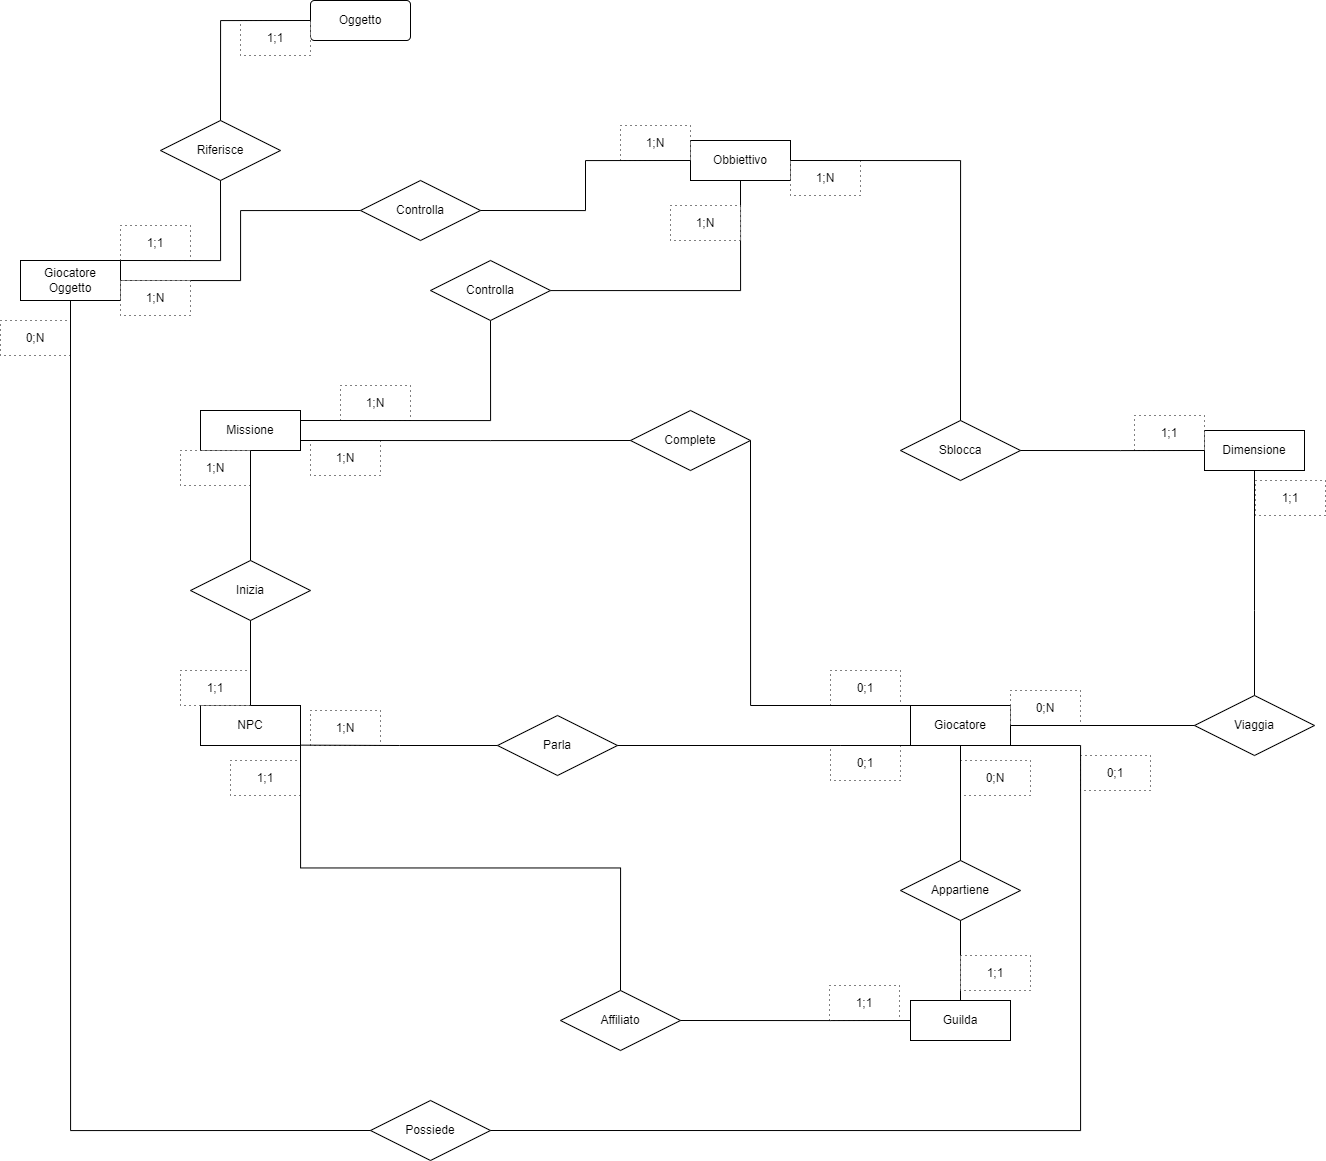
\includegraphics[width=\textwidth]{C:/Users/mutua/Documents/Repository/SQL/Proggetto/vcs.drawio.png}
    \caption{Schema concettuale}
    \label{fig:conceptual_schema}
\end{figure}

\subsection{Relazioni}

\subsubsection{Descrizione delle Relazioni}

\begin{itemize}
    \item \lstinline|giocatore-completa-missione|: Questa relazione indica che un giocatore ha completato una missione specifica.
    \item \lstinline|giocatore-parla-npc|: Questa relazione registra le interazioni tra giocatori e NPC.
    \item \lstinline|giocatore-appartiene-gilda|: Questa relazione denota a quale gilda appartiene un giocatore.
    \item \lstinline|giocatore-possiede-giocatore_oggetto|: Questa relazione indica quali oggetti sono posseduti da un giocatore.
    \item \lstinline|giocatore-viaggia-dimensione|: Questa relazione indica le dimensioni a cui un giocatore ha viaggiato.
    \item \lstinline|gilda-affiliato-npc|: Questa relazione indica l'affiliazione tra gilde e NPC.
    \item \lstinline|npc-inizia-missione|: Questa relazione denota le missioni iniziate dagli NPC.
    \item \lstinline|missione-controlla-obiettivo|: Questa relazione indica le missioni richieste per ottenere obiettivi specifici.
    \item \lstinline|giocatore_oggetto-controlla-obiettivo|: Questa relazione indica quali oggetti del giocatore sono controllati per gli obiettivi.
    \item \lstinline|giocatore_oggetto-riferisce-ogggetto|: Questa relazione denota quali oggetti sono riferiti dagli oggetti del giocatore.
    \item \lstinline|obiettivo-sblocca-dimensione|: Questa relazione indica quali obiettivi sbloccano specifiche dimensioni..
\end{itemize}

\begin{longtable}{|>{\raggedright}m{0.3\textwidth}|>{\centering}m{0.3\textwidth}|>{\raggedright\arraybackslash}m{0.3\textwidth}|}
\hline
\textbf{Entità (0/1;1/n)} & \textbf{Relazione} & \textbf{Entità (0/1;1/n)} \\
\hline
\endfirsthead
\multicolumn{3}{c}{{\bfseries \tablename\ \thetable{} -- continua dalla pagina precedente}} \\
\hline
\textbf{Entità (0/1;1/n)} & \textbf{Relazione} & \textbf{Entità (0/1;1/n)} \\
\hline
\endhead
\hline \multicolumn{3}{|r|}{{Continua alla pagina successiva}} \\ \hline
\endfoot
\hline
\endlastfoot
Giocatore (0/1) & completa & Missione (1/n) \\
\hline
Giocatore (0/1) & Parla & NPC (1/n) \\
\hline
Giocatore (0/n) & appartiene & Gilda (1/1) \\
\hline
Giocatore (0/1) & possiede & Giocatore\_Oggetto (0/n) \\
\hline
Giocatore (0/n) & viaggia & Dimensione (1/1) \\
\hline
Gilda (1/1) & affiliato & NPC (1/1) \\
\hline
NPC (1/1) & inizia & Missione (1/n) \\
\hline
Missione (1/n) & controlla(obiettivo) & Obiettivo (1/n) \\
\hline
Giocatore\_Oggetto (1/n) &  controlla(obiettivo) & Obiettivo (1/n) \\
\hline
Giocatore\_Oggetto (1/1) & riferisce & Oggetto (1/1) \\
\hline
Obiettivo (1/n) & sblocca & Dimensione (1/1) \\
\hline
\end{longtable}

\section{Analisi della ridondanza}

Per analizzare la ridondanza, è importante esaminare le entità e le relazioni per individuare eventuali duplicazioni o dati che possono essere derivati da altre informazioni esistenti. Di seguito è riportata l'analisi di ridondanza per ciascuna entità e relazione:

\subsection*{Entità}

\begin{itemize}
    \item \textbf{Giocatore}: Necessaria per rappresentare i giocatori nel gioco.
    \item \textbf{NPC}: Necessaria per rappresentare i personaggi non giocanti.
    \item \textbf{Gilda}: Necessaria per rappresentare le gilde.
    \item \textbf{Missione}: Necessaria per rappresentare le missioni.
    \item \textbf{Obiettivo}: Necessaria per rappresentare gli obiettivi.
    \item \textbf{Dimensione}: Necessaria per rappresentare le dimensioni del gioco.
    \item \textbf{Oggetto}: Necessaria per rappresentare gli oggetti nel gioco.
    \item \textbf{Giocatore\_Oggetto}: Necessaria per rappresentare gli oggetti posseduti dai giocatori.
\end{itemize}

Non sembra esserci ridondanza, poiché ciascuna di esse rappresenta un concetto distinto nel contesto del gioco.

\subsection*{Relazioni}

\begin{itemize}
    \item \lstinline|giocatore-completa-missione|: Necessaria per tracciare quali missioni sono state completate da ciascun giocatore.
    \item \lstinline|giocatore-parla-npc|: Necessaria per registrare le interazioni tra giocatori e NPC.
    \item \lstinline|giocatore-appartiene-gilda|: Necessaria per denotare l'appartenenza di un giocatore a una gilda.
    \item \lstinline|giocatore-possiede-giocatore_oggetto|: Necessaria per indicare quali oggetti sono posseduti da un giocatore.
    \item \lstinline|giocatore-viaggia-dimensione|: Necessaria per tracciare le dimensioni visitate da un giocatore.
    \item \lstinline|gilda-affiliato-npc|: Necessaria per indicare l'affiliazione tra gilde e NPC.
    \item \lstinline|npc-inizia-missione|: Necessaria per denotare le missioni iniziate dagli NPC.
    \item \lstinline|missione-controlla-obiettivo|: Necessaria per indicare le missioni richieste per ottenere specifici obiettivi.
    \item \lstinline|giocatore_oggetto-controlla-obiettivo|: Necessaria per indicare quali oggetti del giocatore sono controllati per gli obiettivi.
    \item \lstinline|giocatore_oggetto-riferisce-oggetto|: Necessaria per evitare che i giocatori vadano in soft-lock se i loro oggetti non sono nella lista degli oggetti ammessi.
    \item \lstinline|obiettivo-sblocca-dimensione|: Necessaria per indicare quali obiettivi sbloccano specifiche dimensioni.
\end{itemize}

Dopo il chiarimento, nessuna delle relazioni risulta ridondante. Ogni relazione rappresenta un aspetto cruciale delle dinamiche del gioco e non può essere derivata direttamente da altre relazioni senza perdere informazioni importanti.

Dopo l'analisi, non è stata identificata alcuna ridondanza nelle entità e nelle relazioni e perciò lo schema resta uguale

\section{Schema logico}

\subsection{Entità e Attributi}

\begin{longtable}{|>{\raggedright}m{0.3\textwidth}|>{\raggedright\arraybackslash}m{0.6\textwidth}|}
\hline
\textbf{Entità} & \textbf{Attributi} \\
\hline
\endfirsthead
\multicolumn{2}{c}{{\bfseries \tablename\ \thetable{} -- continua dalla pagina precedente}} \\
\hline
\textbf{Entità} & \textbf{Attributi} \\
\hline
\endhead
\hline \multicolumn{2}{|r|}{{Continua alla pagina successiva}} \\ \hline
\endfoot
\hline
\endlastfoot
Giocatore & player\_id (INT, PK), player\_name (VARCHAR), guild\_id (INT, FK) \\
\hline
NPC & npc\_id (INT, PK), npc\_name (VARCHAR), guild\_id (INT, FK) \\
\hline
Gilda & guild\_id (INT, PK), guild\_name (VARCHAR) \\
\hline
Missione & quest\_id (INT, PK), quest\_name (VARCHAR), state (BOOLEAN) \\
\hline
Obiettivo & achievement\_id (INT, PK), achievement\_name (VARCHAR) \\
\hline
Dimensione & dimension\_id (INT, PK), dimension\_name (VARCHAR) \\
\hline
Oggetto & item\_id (INT, PK), item\_name (VARCHAR) \\
\hline
Giocatore\_Oggetto & player\_item\_id (INT, PK), player\_id (INT, FK), item\_id (INT, FK), state (BOOLEAN) \\
\hline
\end{longtable}

\subsection{Relazioni}

\begin{longtable}{|>{\raggedright}m{0.3\textwidth}|>{\raggedright\arraybackslash}m{0.7\textwidth}|}
\hline
\textbf{Relazione} & \textbf{Attributi} \\
\hline
\endfirsthead
\multicolumn{2}{c}{{\bfseries \tablename\ \thetable{} -- continua dalla pagina precedente}} \\
\hline
\textbf{Relazione} & \textbf{Attributi} \\
\hline
\endhead
\hline \multicolumn{2}{|r|}{{Continua alla pagina successiva}} \\ \hline
\endfoot
\hline
\endlastfoot
Completa & player\_id (INT, FK), quest\_id (INT, FK) \\
\hline
Parla & player\_id (INT, FK), npc\_id (INT, FK) \\
\hline
Appartiene & player\_id (INT, FK), guild\_id (INT, FK) \\
\hline
Possiede & player\_id (INT, FK), player\_item\_id (INT, FK) \\
\hline
Viaggia & player\_id (INT, FK), dimension\_id (INT, FK) \\
\hline
Affiliato & guild\_id (INT, FK), npc\_id (INT, FK), affiliation (VARCHAR) \\
\hline
Inizia & npc\_id (INT, FK), quest\_id (INT, FK) \\
\hline
Controlla & quest\_id (INT, FK), player\_id (INT, FK) \\
\hline
Riferisce & player\_item\_id (INT, FK), item\_id (INT, FK) \\
\hline
Sblocca & achievement\_id (INT, FK), dimension\_id (INT, FK) \\
\hline
\end{longtable}

\section{Normalizzazione dello schema logico}

\subsection{Prima Forma Normale (1NF)}

\begin{itemize}
    \item Giocatore: Ogni giocatore ha un unico player\_id, player\_name e guild\_id.
    \item NPC: Ogni NPC ha un unico npc\_id, npc\_name e guild\_id.
    \item Gilda: Ogni gilda ha un unico guild\_id e guild\_name.
    \item Missione: Ogni missione ha un unico quest\_id, quest\_name e state.
    \item Obiettivo: Ogni obiettivo ha un unico achievement\_id e achievement\_name.
    \item Dimensione: Ogni dimensione ha un unico dimension\_id e dimension\_name.
    \item Oggetto: Ogni oggetto ha un unico item\_id e item\_name.
    \item Giocatore\_Oggetto: Ogni oggetto del giocatore ha un unico player\_item\_id, player\_id, item\_id e state.
\end{itemize}

\subsection{Seconda Forma Normale (2NF)}

\begin{itemize}
    \item Giocatore: player\_name e guild\_id dipendono interamente da player\_id.
    \item NPC: npc\_name e guild\_id dipendono interamente da npc\_id.
    \item Gilda: guild\_name dipende interamente da guild\_id.
    \item Missione: quest\_name e state dipendono interamente da quest\_id.
    \item Obiettivo: achievement\_name dipende interamente da achievement\_id.
    \item Dimensione: dimension\_name dipende interamente da dimension\_id.
    \item Oggetto: item\_name dipende interamente da item\_id.
    \item Giocatore\_Oggetto: player\_id, item\_id e state dipendono interamente da player\_item\_id.
\end{itemize}

\subsection{Terza Forma Normale (3NF)}

\begin{itemize}
    \item Giocatore: Non esistono dipendenze transitive.
    \item NPC: Non esistono dipendenze transitive.
    \item Gilda: Non esistono dipendenze transitive.
    \item Missione: Non esistono dipendenze transitive.
    \item Obiettivo: Non esistono dipendenze transitive.
    \item Dimensione: Non esistono dipendenze transitive.
    \item Oggetto: Non esistono dipendenze transitive.
    \item Giocatore\_Oggetto: Non esistono dipendenze transitive.
\end{itemize}

\end{document}
